\section[data]{sPlot / Data-driven Techniques}

\begin{frame}
    \frametitle{Reweighting}
    \begin{center}
        \begin{itemize}
            \item Requires MC and data events
            \item Train classifier to distinguish data events and MC events
            \item Reweight MC events using output of classifier
            \item Train classifier to distinguish signal and background using reweighted MC
        \end{itemize}
    \end{center}
\end{frame}

\begin{frame}
    \frametitle{Side-band Subtraction}
    \begin{center}
        \begin{itemize}
            \item Requires number of events in signal region and sideband
            \item Compensates background events in signal region with negative signal events from the sideband
        \end{itemize}
        \begin{tikzpicture}
            \node[anchor=south west,inner sep=0] (image) at (0,0) {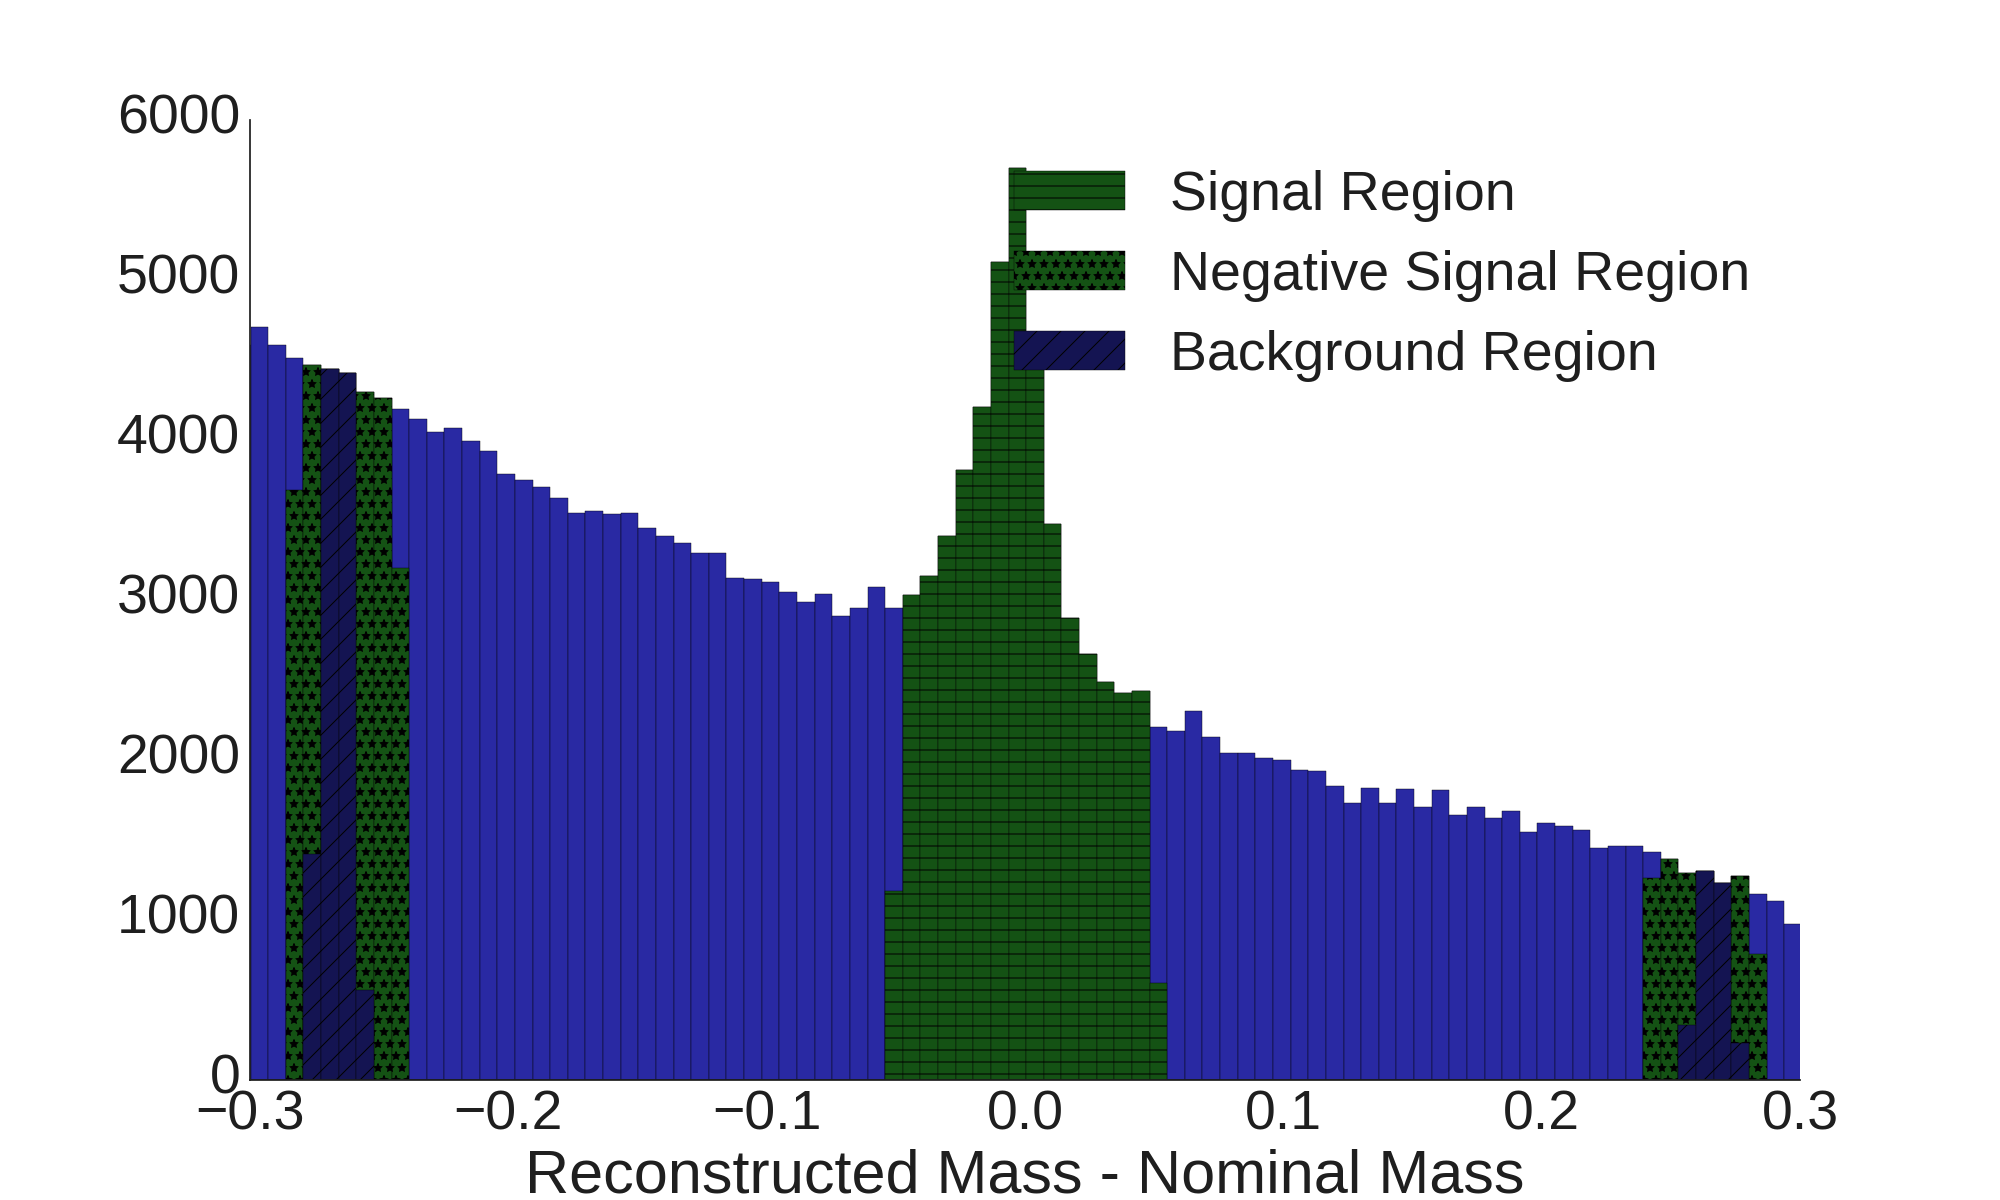
\includegraphics[width=0.7\textwidth]{sideband.png}};
        \end{tikzpicture}
    \end{center}
\end{frame}

\begin{frame}
    \frametitle{sPlot}
    \begin{center}
        \begin{itemize}
            \item Requires yields and covariance of fitted signal + background model
            \item Uses every event twice, as signal and as background with sPlot weight
        \end{itemize}
        \vspace{-1em}


        \begin{align*}
          w(\vec{x}_i) &= \frac{ V_{SS} PDF(\vec{x}_i | S) +  V_{SB} PDF(\vec{x}_i | B)} {N_S  PDF(\vec{x}_i | S) +  N_{B} PDF(\vec{x}_i | B)}
        \end{align*}
        \vspace{-1em}


        \begin{tikzpicture}
            \node[anchor=south west,inner sep=0] (image) at (0,0) {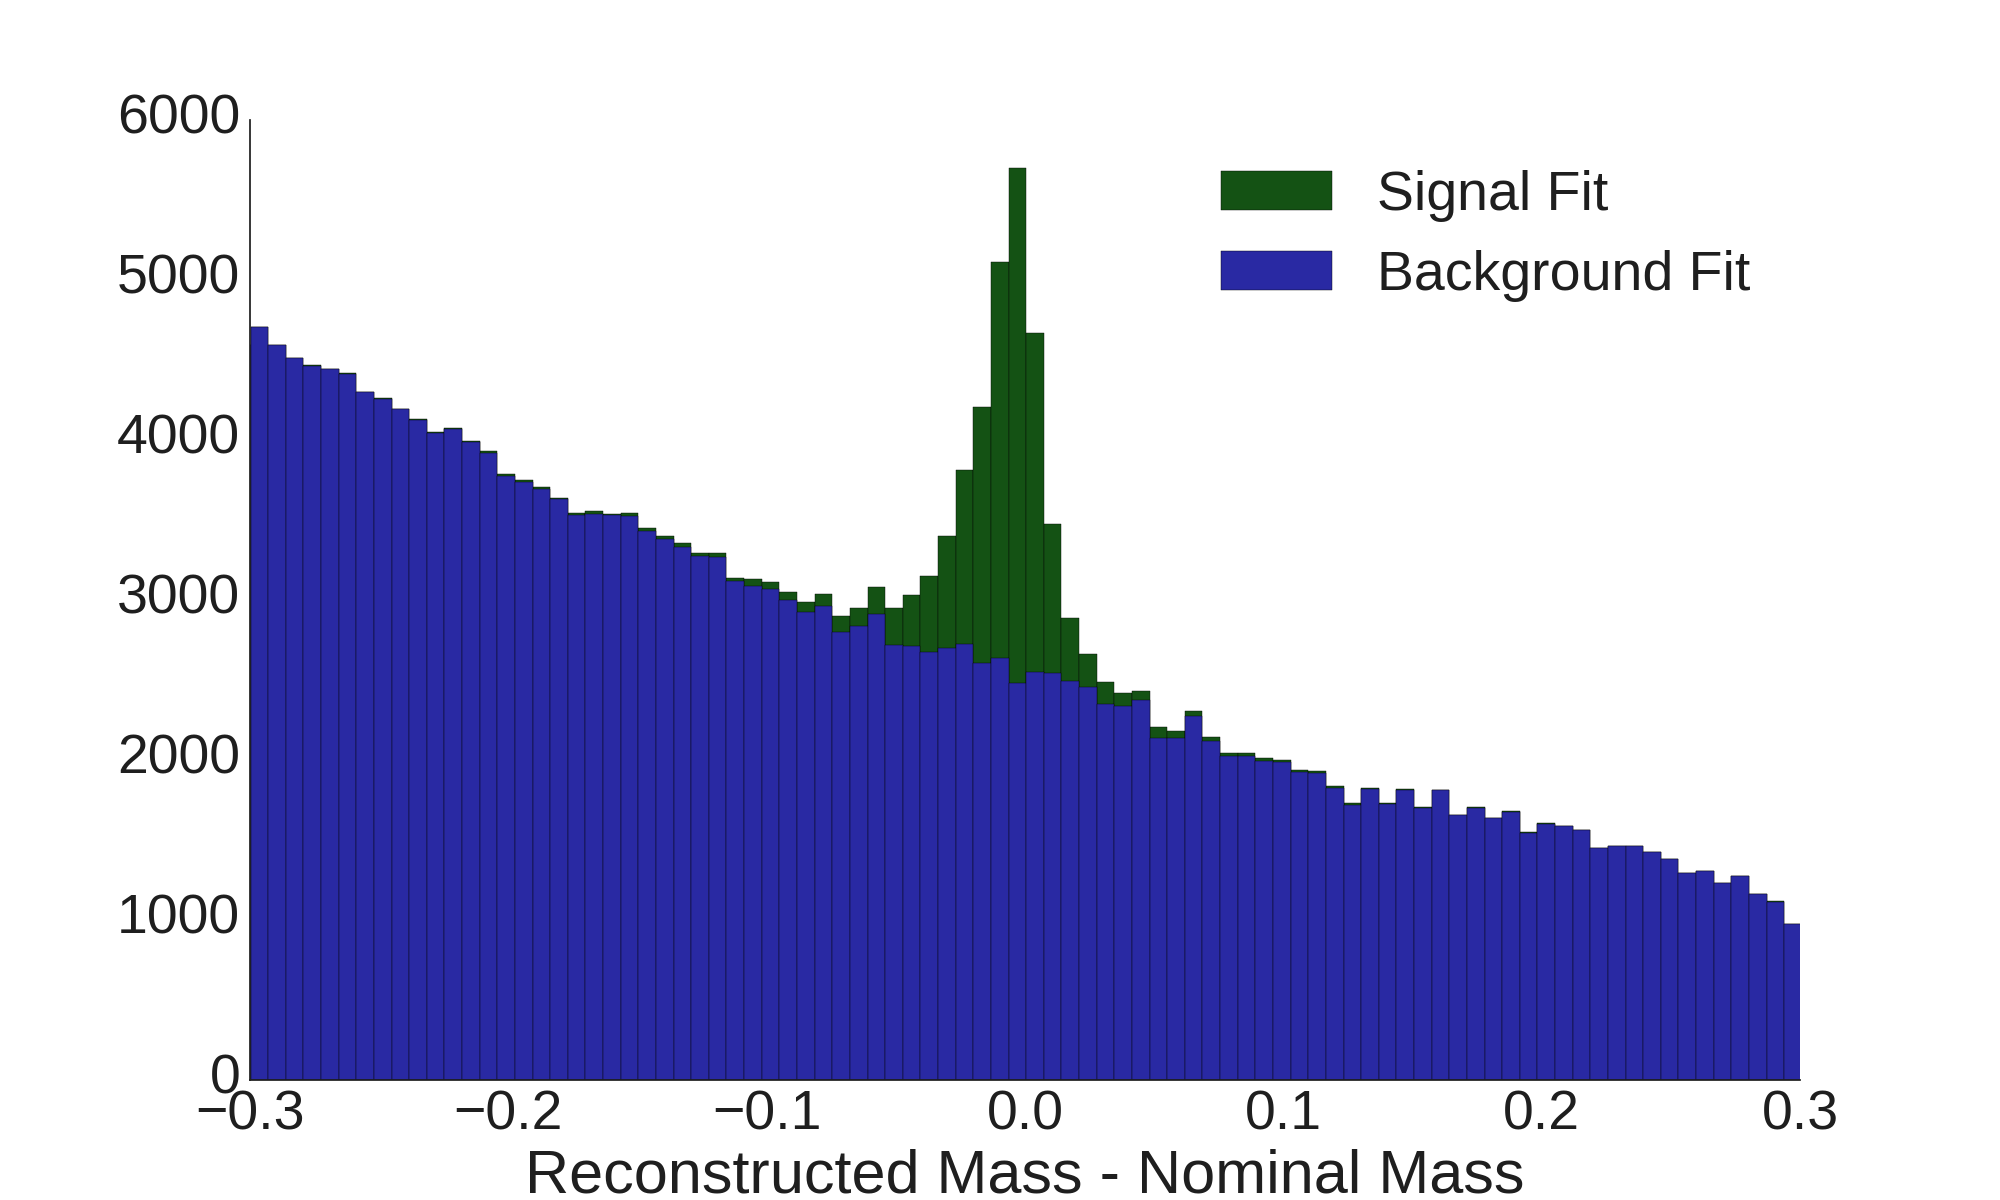
\includegraphics[width=0.7\textwidth]{splot.png}};
        \end{tikzpicture}
    \end{center}
\end{frame}

\begin{frame}
    \frametitle{Example Classifier Quality}
    \begin{center}
        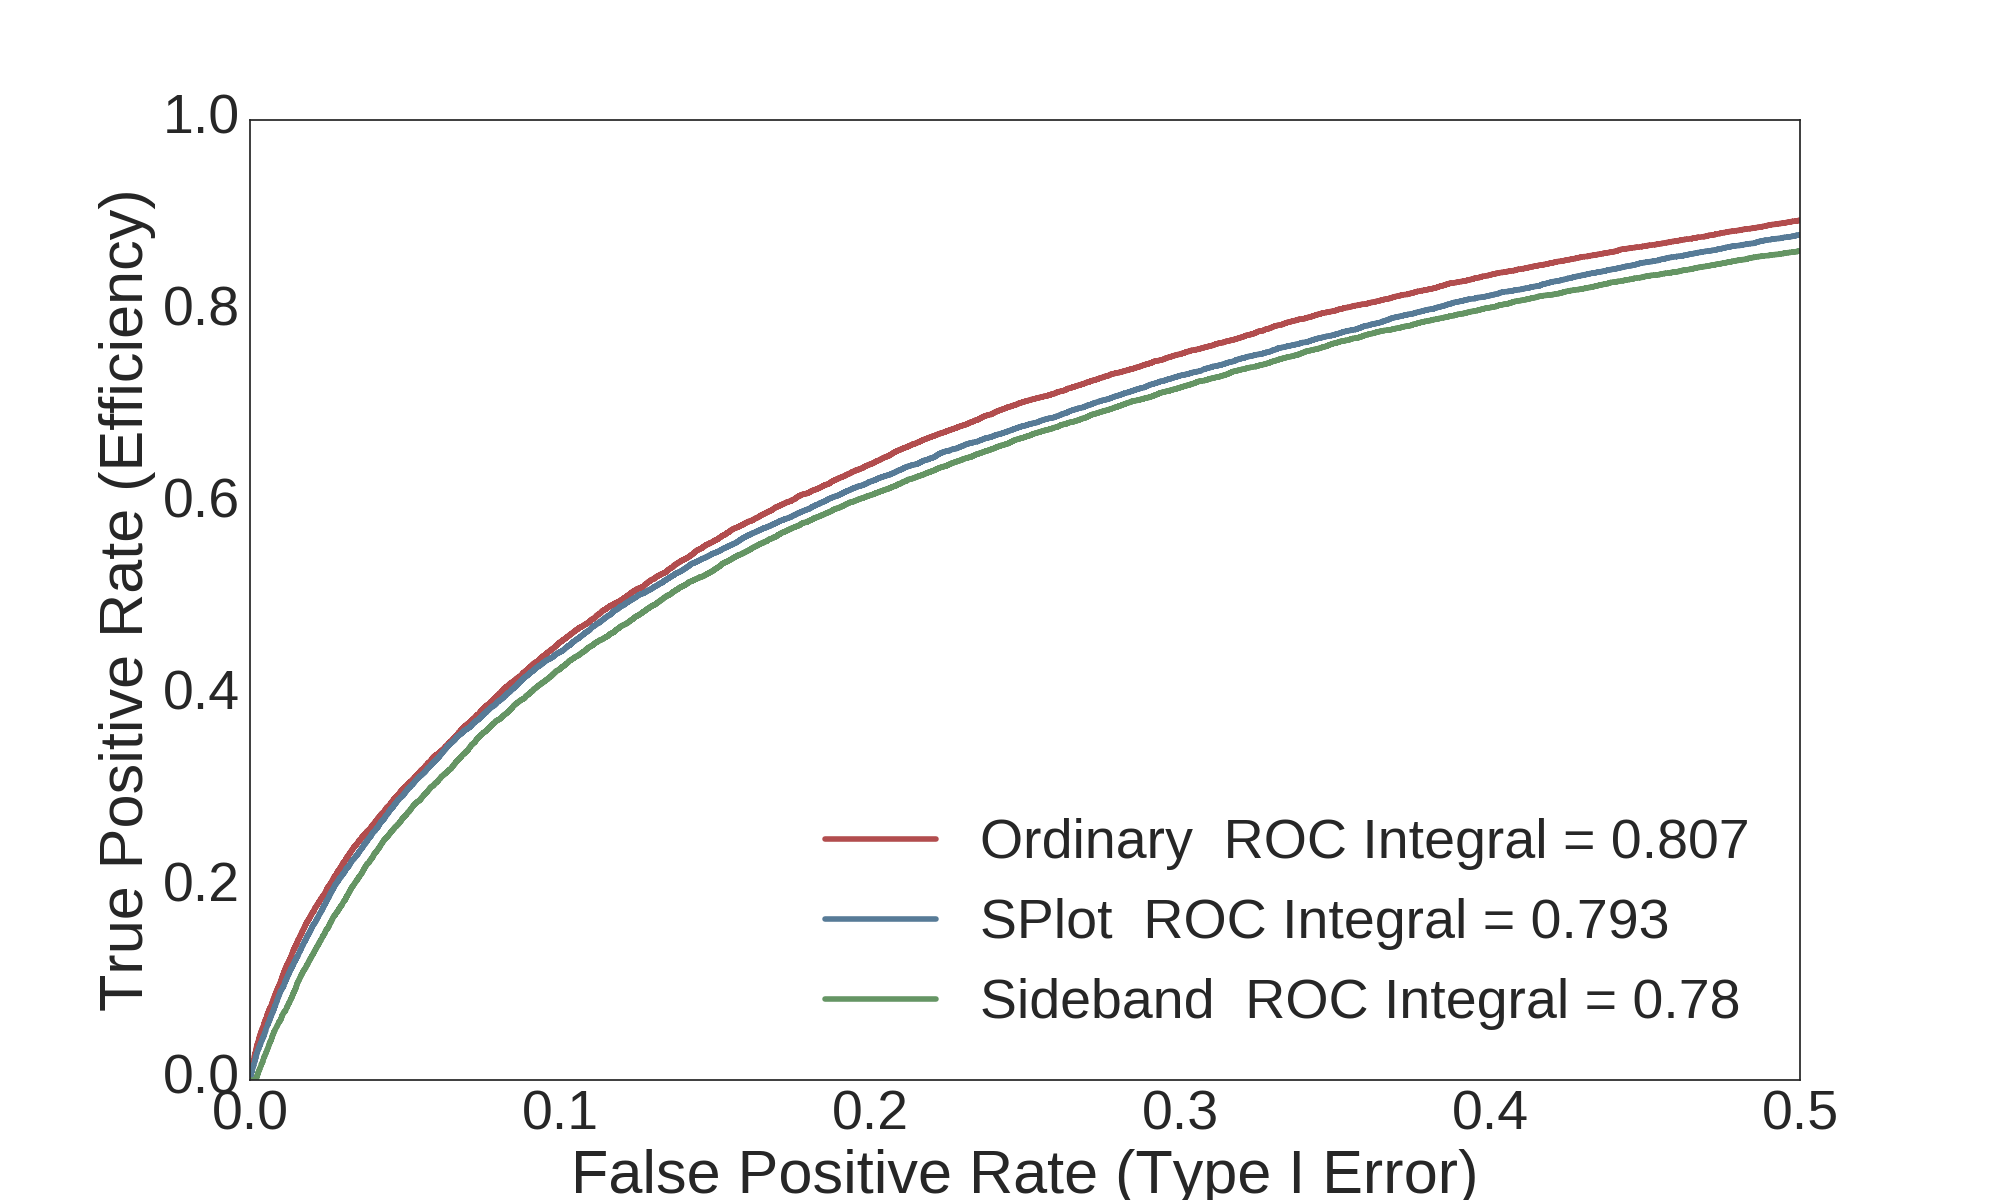
\includegraphics[width=\textwidth]{splot_sideband_roc.png}
    \end{center}
\end{frame}

